\documentclass[12pt]{article}

% Ustawienia strony
\usepackage{lipsum}
\usepackage[margin=1.5cm]{geometry}
\usepackage{graphicx}
\usepackage{enumitem}
\usepackage{siunitx}
\usepackage{amsmath}
\usepackage{cancel}
\usepackage{makecell}
\usepackage{mathtools}
\usepackage{floatrow}
\usepackage{caption}
\usepackage[T1]{fontenc}
\usepackage{fancyvrb}
\usepackage[ngerman]{babel} %Deutsche Sprachunterstützung
\usepackage{subcaption}
\usepackage{graphicx}
\usepackage{blindtext}
\usepackage{hyperref}

\hypersetup{
	colorlinks=true,
	linkcolor=blue,
	filecolor=magenta,      
	urlcolor=cyan,
	pdftitle={Overleaf Example},
	pdfpagemode=FullScreen,
}

\urlstyle{same}

\fvset{tabsize=4}
\setlist{leftmargin=15pt,labelindent=15pt}
\setlist[enumerate]{noitemsep,wide=0pt, leftmargin=*}
{\setlength{\parindent}{0pt}

% Ustawienia stopki
\usepackage{lastpage}
\usepackage{fancyhdr}
\pagestyle{fancy}
\fancyhf{} % sets both header and footer to nothing
\renewcommand{\headrulewidth}{0pt}
\cfoot{\thepage\ z \pageref*{LastPage}}

\begin{document}

\section*{Podstawowe dane}
\begin{figure}[htp]
	\begin{minipage}[t]{0.3\textwidth}
		\textbf{Imie i nazwisko} \\
		\textbf{Data} \\
		\textbf{Tytuł} \\
		\textbf{Numer ćwiczenia}
	\end{minipage}%
	\begin{minipage}[t]{0.6\textwidth}
		Robert Mesek \\
		01.11.2023 \\
		Algorytmy geometryczne \\
		2
	\end{minipage}%
\end{figure}

\section*{Dane techniczne}
\begin{figure}[htp]
	\begin{minipage}[t]{0.3\textwidth}
		\textbf{Procesor} \\
		\textbf{Język} \\
		\textbf{Biblioteki} \\
		\textbf{System operacyjny} \\
		\textbf{Środowisko}

	\end{minipage}%
	\begin{minipage}[t]{0.6\textwidth}
		Intel i7-1165G7 x86\_64 \\
		Python 3.11.5 \\
		NumPy 1.26.0, Pandas 2.1.1, Matplotlib 3.8.0 \\
		WSL Ubuntu 22.04 (MS Windows 10 22H2) \\
		conda 23.5.2
	\end{minipage}%
\end{figure}

\subsection*{Czym jest otoczka wypukła?}
\begin{figure}[htp]
	\begin{minipage}[t]{0.5\textwidth}
		\vspace{1em}
		
		Podzbiór płaszczyzny $Q$ nazywamy wypukłym $\iff$, gdy dla dowolnej pary punktów $p, q \in Q$ odcinek $\overline{pq}$ jest całkowicie zawarty w $Q$.  
		Otoczka wypukła $\mathcal{CH}(Q)$ zbioru $Q$ jest najmniejszym wypukłym zbiorem zawierającym $Q$.
	\end{minipage}%
	\hfill
	\begin{minipage}[t]{0.5\textwidth}
		\centering
		\vspace{0pt}
		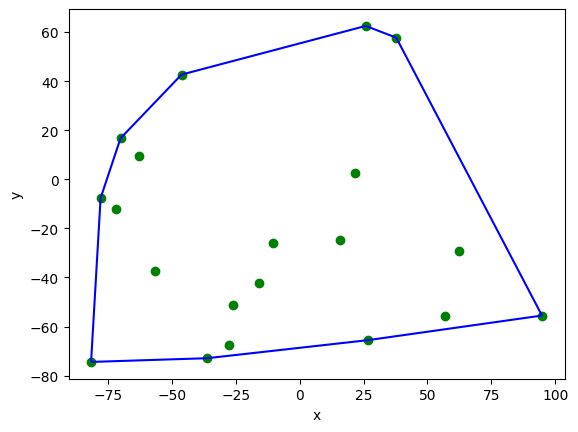
\includegraphics[width=1\linewidth]{images/przyklad.png}
		
		
	\end{minipage}%
	\hspace*{\fill}
\end{figure}

\subsection*{Zastosowania otoczku wypukłej} 
Otoczki wypukłe - w szczególności otoczki wypukłe w przestrzeni trójwymiarowej - są spotykane w różnych zastosowaniach. Na przykład używa się ich do przyspieszania wykrywania kolizji w animacji komputerowej. Przepuśćmy, że chcemy sprawdzić, czy dwa obiekty $\mathcal{P_1}$ i $\mathcal{P_2}$ przecinają się. Jeśli przez większość czasu odpowiedź na to pytanie jest negatywna, to opłaca się następująca strategia. Przybliżamy obiekty przez prostsze obiekty $\widehat{\mathcal{P_1}}$ i $\widehat{\mathcal{P_2}}$, które zawierały oryginały. Jeśli chcemy sprawdzić, czy $\mathcal{P_1}$ i $\mathcal{P_2}$ przecinają się, najpierw sprawdzamy, czy przecinają się $\widehat{\mathcal{P_1}}$ i $\widehat{\mathcal{P_2}}$. Jeśli występuje ten przypadek, to powinniśmy wykonać test na oryginalnych obiektach, który jest przepuszczanie znacznie kosztowniejszy.  
Sprawdzanie przecięcia otoczek wypukłych jest bardziej skomplikowane niż dla sfer - choć mimo to łatwiejsze niż dla obiektów niewypukłych - ale otoczki wypukłe mogą dużo lepiej przybliżać większość obiektów.

\newpage

\subsection*{Zbiory punktów}
\par
\verb|points_a| \\
$100$ losowych punktów w przestrzeni 2D o współrzędnych z przedziału $x \in \langle -100,100 \rangle$ oraz $y \in \langle -100,100\rangle$.
\begin{figure}[H]
	\centering
	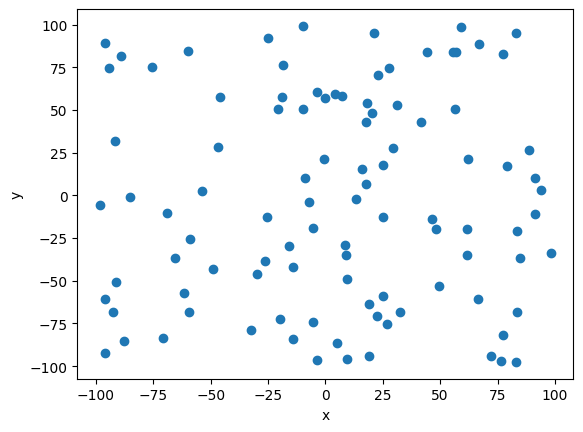
\includegraphics[width=0.7\linewidth]{images/zbior-a.png}
\end{figure}

\verb|points_b| \\
$100$ losowych punktów w przestrzeni 2D leżących na okręgu o środku $O = (0,0)$ i promieniu $R = 10$.
\begin{figure}[H]
	\centering
	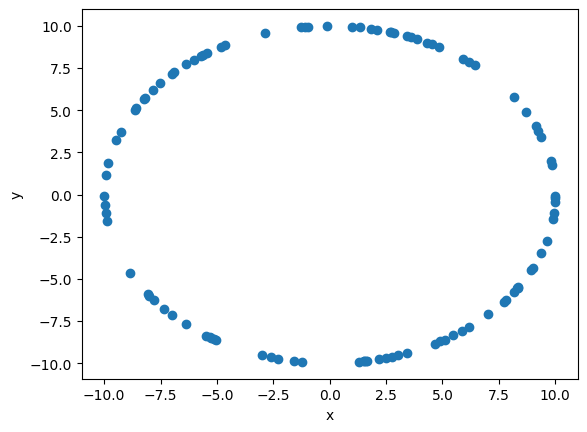
\includegraphics[width=0.7\linewidth]{images/zbior-b.png}
\end{figure}

\newpage

\par
\verb|points_c| \\
$100$ losowych punktów w przestrzeni 2D leżących na obwodzie prostokąta, którego wyznaczają wierzchołki
$(-10,-10), (10,-10), (10,10)$ oraz $(-10,10)$.
\begin{figure}[H]
	\centering
	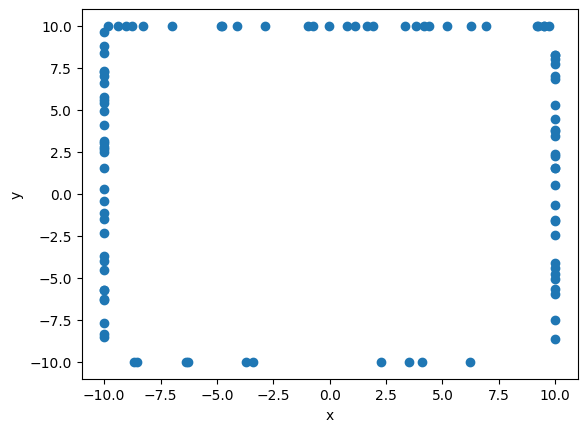
\includegraphics[width=0.7\linewidth]{images/zbior-c.png}
\end{figure}

\par
\verb|points_d| \\
po 25 punktów na dwóch bokach kwadratu leżących na osiach i po 20 punktów na przekątnych kwadratu, zawierający punkty wyznaczające kwadrat $(0, 0), (10, 0), (10, 10)$ oraz $(0, 10)$.
\begin{figure}[H]
	\centering
	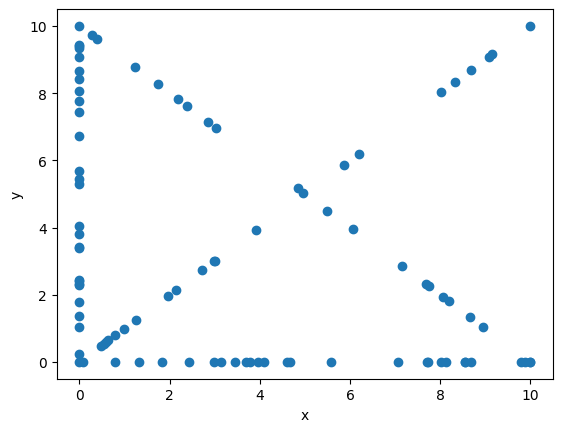
\includegraphics[width=0.7\linewidth]{images/zbior-d.png}
\end{figure}

\newpage

\section*{Algorytm Grahama oraz algorytm Jarvisa}
\subsection*{Funkcje pomocnicze dla obu algorytmów}

\par Reprezentuje punkt
\begin{Verbatim}
class Point:
	def __init__(self, x, y, id=None):
		self.x = x
		self.y = y
		self.id = id  # set to index
	
	def __repr__(self):
		return f"{self.id}. ({self.x}, {self.y})"
	
	def as_tuple(self):
		return (self.x, self.y)
\end{Verbatim}

\mbox{}
\par Konwertuje listę krotek na listę punktów
\begin{Verbatim}
def create_points(Q: list[tuple]):
	points = []
	for i, (x, y) in enumerate(Q):
		points.append(Point(x, y, i))
	return points
\end{Verbatim}

\mbox{}
\par Konwertuje listę punktów na listę krotek
\begin{Verbatim}
def to_list_of_tuples(points: list[Point]):
	list_of_tuples = []
	for point in points:
		list_of_tuples.append(point.as_tuple())
	return list_of_tuples
\end{Verbatim}

\mbox{}
\par Sprawdza orientację punktu względem prostej korzystając z wyznacznika macierzy
\begin{Verbatim}
def find_orient(a: Point, b: Point, c: Point):
	"""
	Orientacja punktu "c" względem prostej "a b" obliczając wyznacznik macierzy 2x2
	:param a: pierwszey punkt tworzący naszą prostą
	:param b: drugi punkt tworzący naszą prostą
	:param c: punkt, którego położenie względem prostej chcemy znaleźć
	:return: wartość wyznacznika macierzy
	(> 0) => Counterclockwise
	(== 0) => Collinear
	(< 0) => Clockwise
	"""
	return (a.x - c.x) * (b.y - c.y) - (a.y - c.y) * (b.x - c.x)
\end{Verbatim}

\newpage

\par Oblicza odległość punktów
\begin{Verbatim}
def distance(p1: Point, p2: Point):
	return ((p2.x - p1.x) ** 2 + (p2.y - p1.y) ** 2) ** 0.5
\end{Verbatim}

\mbox{}
\subsection*{Funkcje pomocnicze dla algorytmu grahama}

\par Zwraca punkt startowy dla algorytmu
\begin{Verbatim}
def find_start_point(points: list[Point]):
	return min(points, key=lambda p: (p.y, p.x))
\end{Verbatim}

\mbox{}
\par Sortuje punkty względem kąta jaki tworzą z prostą OX
\begin{Verbatim}
def sort_points(p0: Point, points: list[Point], eps):
	from functools import cmp_to_key
	
	def compare(p1: Point, p2: Point, cmp_eps=eps):
		"""Will return a negative value for less-than, zero if the inputs are equal, 
		or a positive value for greater-than"""
		orient = find_orient(p1, p2, p0)
		if abs(orient) < cmp_eps:
			if distance(p0, p1) > distance(p0, p2):
				p2.id = None  # None if collinear
				return 1
			else:
				p1.id = None  # None if collinear
				return -1
		elif orient > 0:
			return -1
		else:
			return 1

	points.sort(key=cmp_to_key(compare))
\end{Verbatim}

\mbox{}
\par Usuwa punkty współliniowe wykorzystując flagę nadaną podczas sortowania
\begin{Verbatim}
def remove_collinear(points: list[Point]):
	for i in reversed(range(len(points))):
		if points[i].id is None:
			points.pop(i)
\end{Verbatim}

\newpage

\subsection*{Algorytm Grahama}
Algorytm Grahama tworzy otoczkę wypukłą poprzez utrzymywanie stosu $S$, w którym znajdują się punkty, które mogą, ale nie muszą tworzyć otoczki wypukłej. Za każdym razem jest wstawiany na stos (push) jeden punkt z zbioru punktów $Q$ i jest on usuwany ze stosu (pop), jeżeli nie jest punktem $\mathcal{CH}(Q)$. Kiedy algorytm kończy się, stos $S$ zawiera tylko punkty otoczki wypukłej $\mathcal{CH}(Q)$ w kierunku przeciwnym do ruchu wskazówek zegara.

---

Procedura $\mathtt{Graham-Build(Q)}$ przyjmuje zbiór punktów $Q$, gdzie $|Q| \geq 3$. Wywołuje ona funkcję $\mathtt{TOP(S)}$, która zwraca punkt z góry stosu bez zmieniania $S$ oraz
$\mathtt{NEXT-TO-TOP(S)}$, która zwraca punkt poniżej góry stosu $S$, bez zmieniania stosu. Funkcja $\mathtt{PUSH(p, S)}$ wstawia punkt $p$ na stos $S$. Funkcja $\mathtt{POP(p, S)}$ usuwa punkt $p$ ze stosu $S$.


\mbox{}\newline
$\mathtt{Graham-Build(Q)}$  

1)  niech $p_0$ będzie punktem w zbiorze Q z najmniejszą współrzędną $y$,  
oraz najmniejszą współrzędną $x$ w przypadku, gdy wiele punktów ma tą samą współrzędną $x$  


2)  nich $\mathtt{\langle p_1, p_2, \dots, p_m \rangle}$ będzie pozostałym zbiorem punktów w $Q$ posortowanym  
zgodnie z przeciwnym ruchem wskazówek zegara wokół punktu $p_0$  
(jeżeli więcej niż jeden punkt ma ten sam kąt to usuwamy wszystkie punkty  
z wyjątkiem tego najbardziej oddalonego od $p_0$)  


3) stwórz pusty stos $S$  


4) $\mathtt{PUSH(p_0, S)}$


5) $\mathtt{PUSH(p_1, S)}$


6) $\mathtt{PUSH(p_2, S)}$


7) \textbf{for} $i = 3$ \textbf{to} m  


8) \quad\textbf{while} kąt utworzony przez $\mathtt{NEXT-TO-TOP(S)}$, $\mathtt{TOP(S)}$ oraz $p_i$ tworzy lewostronny skręt


9) \quad\quad$\mathtt{POP(S)}$


10) \quad$\mathtt{PUSH(p_i, S)}$


11) \textbf{return} $S$

\begin{Verbatim}
def graham_algorithm(Q, eps=10**-24):
	"""
	Funkcja buduje otoczkę wypukłą dla podanego
	zbioru punktów Q algorymem Grahama
	:parm Q: zbiór punktów
	:return: tablica punktów w postaci krotek współrzędnych
	"""
	points = create_points(Q)
	start_point = points.pop(find_start_point(points).id)
	sort_points(start_point, points, eps)
	remove_collinear(points)  # according to angle (start_point -> a), (start_point -> b)
	stack = [start_point]
	for point in points:
		while len(stack) > 1 and find_orient(stack[-2], stack[-1], point) <= 0:
			stack.pop()
		stack.append(point)
	return to_list_of_tuples(stack)
\end{Verbatim}

\newpage

\section*{Analiza wyników}
\subsection*{Znaczenie kolorów}
Niebieskie punkty - cały zbiór; Zielone punkty -  rozpatrywane punkty przez algorytm, po usunięciu współliniowych; czerwona linia - aktualnie rozpatrywana krawędź; niebieska linia - znaleziona otoczka wypukła.

\subsection*{Zbiór A}
\begin{figure}[htp]
	\begin{subfigure}[t]{.45\textwidth}
		\centering
		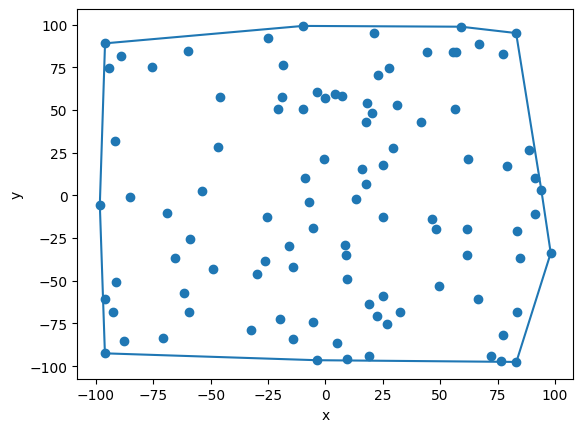
\includegraphics[width=\linewidth]{images/graham-a.png}
		\caption*{Rysunek Graham points\_a}
	\end{subfigure}
	\hfill
	\begin{subfigure}[t]{.45\textwidth}
		\centering
		\href{images/graham-a.gif}{images/graham-a.gif}
		\caption*{Animacja Graham points\_a}
	\end{subfigure}
\end{figure}

\subsection*{Zbiór B}
\begin{figure}[htp]
	\begin{subfigure}[t]{.45\textwidth}
		\centering
		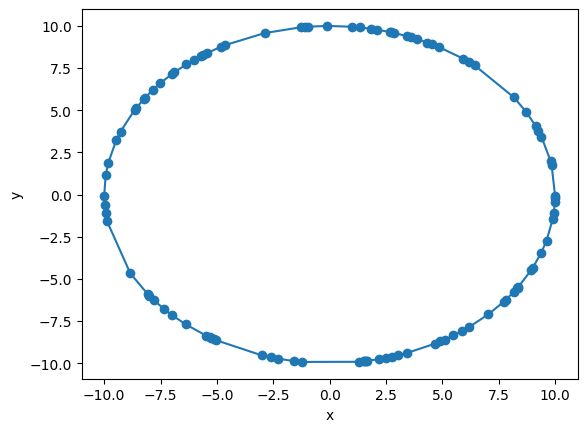
\includegraphics[width=\linewidth]{images/graham-b.png}
		\caption*{Rysunek Graham points\_b}
	\end{subfigure}
	\hfill
	\begin{subfigure}[t]{.45\textwidth}
		\centering
		\href{images/graham-b.gif}{images/graham-b.gif}
		\caption*{Animacja Graham points\_b}
	\end{subfigure}
\end{figure}

\newpage

\subsection*{Zbiór C}
\begin{figure}[htp]
	\begin{subfigure}[t]{.45\textwidth}
		\centering
		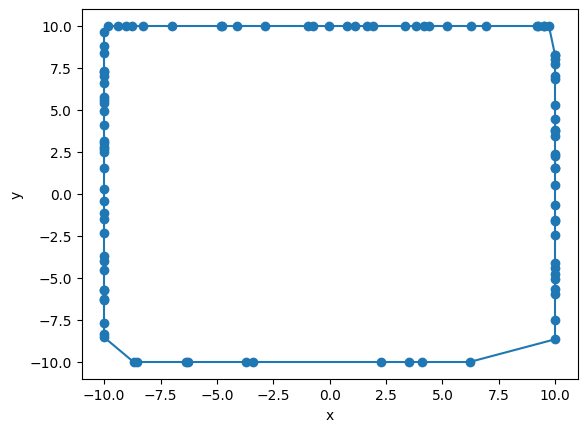
\includegraphics[width=\linewidth]{images/graham-c.png}
		\caption*{Rysunek Graham points\_c}
	\end{subfigure}
	\hfill
	\begin{subfigure}[t]{.45\textwidth}
		\centering
		\href{images/graham-c.gif}{images/graham-c.gif}
		\caption*{Animacja Graham points\_c}
	\end{subfigure}
\end{figure}

\subsection*{Zbiór D}
\begin{figure}[htp]
	\begin{subfigure}[t]{.45\textwidth}
		\centering
		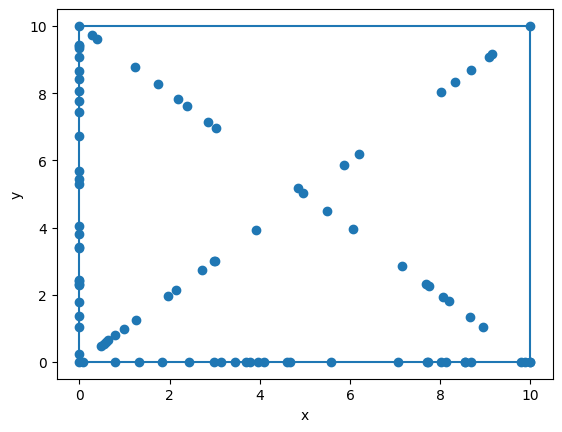
\includegraphics[width=\linewidth]{images/graham-d.png}
		\caption*{Rysunek Graham points\_d}
	\end{subfigure}
	\hfill
	\begin{subfigure}[t]{.45\textwidth}
		\centering
		\href{images/graham-d.gif}{images/graham-d.gif}
		\caption*{Animacja Graham points\_d}
	\end{subfigure}
\end{figure}

\paragraph{Wnioski:}
\mbox{}\newline
Analizując wyniki, widzimy że algorytm grahama dosyć dokładnie wyznaczył otoczki wypukłe dla wszystkich zbiorów.

Widzimy jednak, że usuwanie punktów współliniowych względem kąta jaki tworzą z osią OX, nie jest idealne.
Dla zbioru C z powodu punktu punktu startowego, została odrzucona jedynie dolna krawędź, więc operacja odrzucania krawędzi nie zaoszczędziła dużo w tym przypadku. Zbiór D lepiej pokazuje, które punkty zostaną początkowo usunięte (bok ab oraz ad oraz proste wychodzące z punktu a).

Kolejnym problemem z jakim możemy się spotkać jest fakt, że decydując, który punkt zostanie wybrany porównujemy ich kąty, więc zmiana epsilon, nie wpływa w intuicyjny sposób na zwiększanie dokładności.
\newpage

\subsection*{Funkcje pomocnicze dla algorytmu jarvisa}
\par Zwraca punkt startowy dla algorytmu
\begin{Verbatim}
def find_start_point(points: list[Point]):
	return min(points, key=lambda p: (p.x, p.y))
\end{Verbatim}

\mbox{}
\par Szuka kolejnego punktu kierując się kątem jaki tworzą z ostatnim punktem na otoczce, a w przypadku odcinków współliniowych wybiera najdalszy.
\begin{Verbatim}
def find_next_point(start_point: Point, points: list[Point], eps):
	end_point = points[0]
	for point in points[1:]:
		orient = find_orient(start_point, end_point, point)
		if abs(orient) < eps and distance(start_point, point) > distance(start_point, end_point):
			end_point = point
		elif orient < 0:
			end_point = point
	return end_point
\end{Verbatim}


\subsection*{Algorytm Jarvisa}
Algorytm Jarvisa oblicza otoczkę wypukłą dla zbioru punktów $Q$ przez technikę zwaną owijaniem paczki (\textbf{package wrapping}) lub owijaniem prezentu (\textbf{gift wrapping}). Algorytm Jarvisa buduje sekwencję $H = \langle p_1, p_2, \dots, p_m \rangle$ będącą wierzchołkami $\mathcal{CH}(Q)$. Zaczynamy od punktu $p_0$, następny punkt $p_1$ w otoczce wypukłej ma najmniejszy kąt w odniesieniu do $p_0$ (w przypadku takiego samego kąta - wybiera się punkt najdalej od $p_0$). Podobnie, gdy $p_2$ ma najmniejszy kąt w odniesieniu do $p_1$, itd.. Zauważyć warto, że możemy tym sposobem obliczyć lewy i prawy łańcuch otoczki wypukłej $\mathcal{CH}(Q)$. Lewy łańcuch buduje się podobnie. Gdy osiągniemy najwyższy wierzchołek w prawym łańcuchu $p_k$, wybieramy wierzchołek $p_{k+1}$, który ma najmniejszy kąt w odniesieniu do $p_k$, ale od ujemnej osi-$x$. Można zaimplementować algorytm Jarvisa bez konstruowania pomocniczych łańcuchów - lewego i prawego. Taka implementacja utrzymuje śledzenie kąta ostatniej strony otoczki wypukłej i wymaga sekwencji kątów boków otoczki tylko rosnącej. (Patrząc na trzy ostatnie punkty jesteśmy w stanie obliczyć jaki punkt należy włączyć do $\mathcal{CH}(Q)$ w zależności od budowanego punktu)

\begin{Verbatim}
def jarvis_algorithm(Q, eps=10**-24):
	"""
	Funkcja buduje otoczkę wypukłą dla podanego
	zbioru punktów Q algorymem Jarvisa
	:parm Q: zbiór punktów
	:return: tablica punktów w postaci krotek współrzędnych
	"""
	points = create_points(Q)
	hull = [find_start_point(points)]
	for _ in range(len(points)):
		next_point = find_next_point(hull[-1], points, eps)
		if distance(hull[0], next_point) < eps:
			break
	hull.append(next_point)
	return to_list_of_tuples(hull)
\end{Verbatim}

\newpage

\section*{Analiza wyników}
\subsection*{Znaczenie kolorów}
Niebieskie punkty - cały zbiór punktów; czerwona linia - aktualnie rozpatrywana krawędź; niebieska linia - znaleziona otoczka wypukła.

\subsection*{Zbiór A}
\begin{figure}[htp]
	\begin{subfigure}[t]{.45\textwidth}
		\centering
		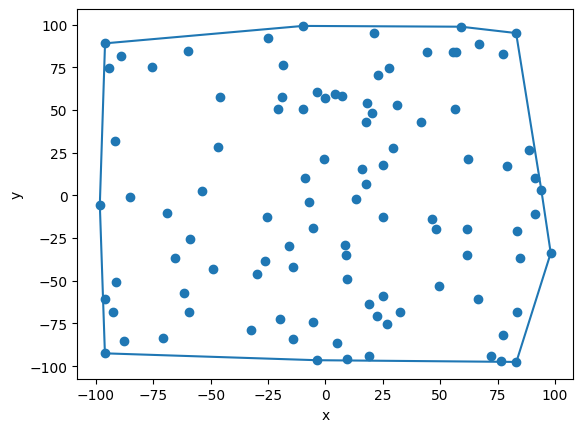
\includegraphics[width=\linewidth]{images/jarvis-a.png}
		\caption*{Rysunek Jarvis points\_a}
	\end{subfigure}
	\hfill
	\begin{subfigure}[t]{.45\textwidth}
		\centering
		\href{images/jarvis-a.gif}{images/jarvis-a.gif}
		\caption*{Animacja Jarvis points\_a}
	\end{subfigure}
\end{figure}

\subsection*{Zbiór B}
\begin{figure}[htp]
	\begin{subfigure}[t]{.45\textwidth}
		\centering
		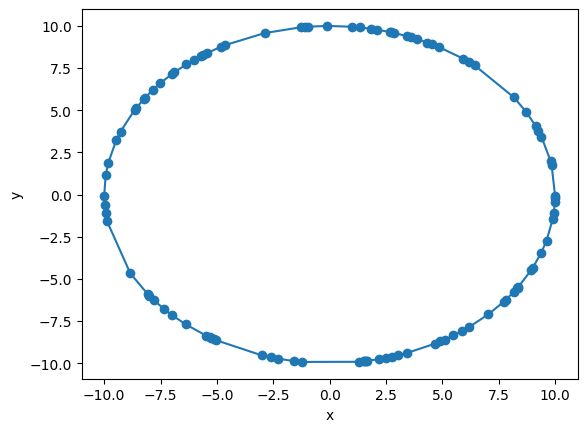
\includegraphics[width=\linewidth]{images/jarvis-b.png}
		\caption*{Rysunek Jarvis points\_b}
	\end{subfigure}
	\hfill
	\begin{subfigure}[t]{.45\textwidth}
		\centering
		\href{images/jarvis-b.gif}{images/jarvis-b.gif}
		\caption*{Animacja Jarvis points\_b}
	\end{subfigure}
\end{figure}

\newpage

\subsection*{Zbiór C}
\begin{figure}[htp]
	\begin{subfigure}[t]{.45\textwidth}
		\centering
		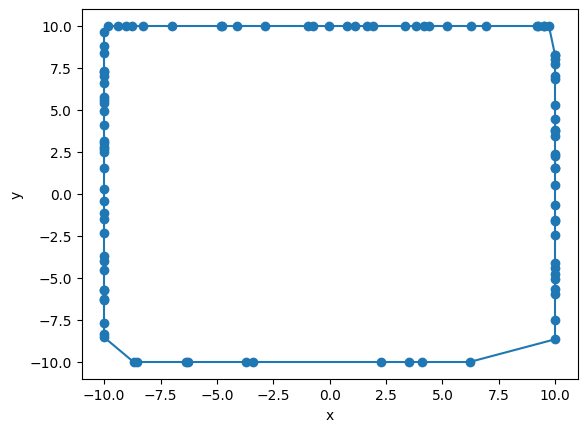
\includegraphics[width=\linewidth]{images/jarvis-c.png}
		\caption*{Rysunek Jarvis points\_c}
	\end{subfigure}
	\hfill
	\begin{subfigure}[t]{.45\textwidth}
		\centering
		\href{images/jarvis-c.gif}{images/jarvis-c.gif}
		\caption*{Animacja Jarvis points\_c}
	\end{subfigure}
\end{figure}

\subsection*{Zbiór D}
\begin{figure}[htp]
	\begin{subfigure}[t]{.45\textwidth}
		\centering
		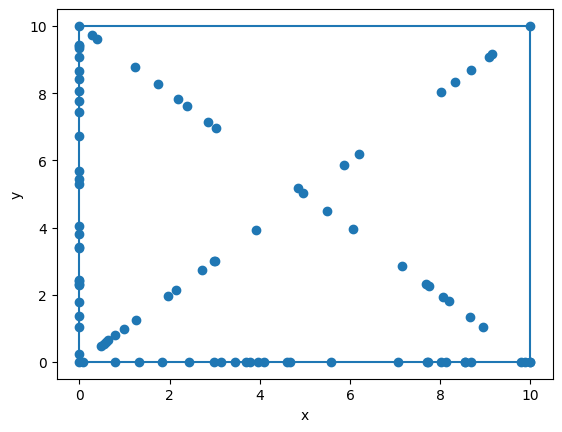
\includegraphics[width=\linewidth]{images/jarvis-d.png}
		\caption*{Rysunek Jarvis points\_d}
	\end{subfigure}
	\hfill
	\begin{subfigure}[t]{.45\textwidth}
		\centering
		\href{images/jarvis-d.gif}{images/jarvis-d.gif}
		\caption*{Animacja Jarvis points\_d}
	\end{subfigure}
\end{figure}

\paragraph{Wnioski:}
\mbox{}\newline
Analizując wyniki, widzimy że algorytm jarvisa wyznaczył dokładnie otoczki wypukłe dla wszystkich zbiorów.

Wybór punktów jest realizowany w intuicyjny sposób.

\newpage
\section*{Zbiory wykorzystane przy porównywaniu czasu działania}

\begin{figure}[htp]
	\begin{subfigure}[t]{.45\textwidth}
		\centering
		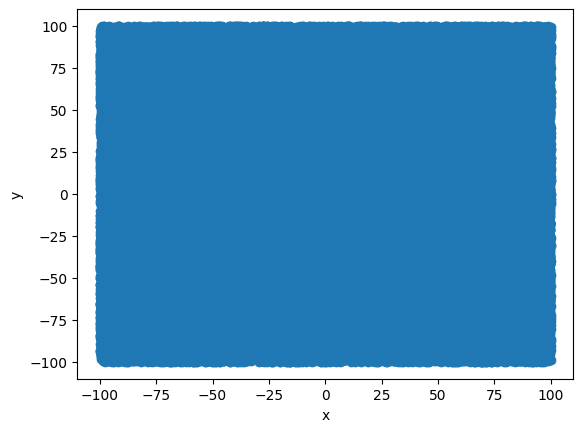
\includegraphics[width=\linewidth]{images/d-zbior-a.png}
		\verb|generate_uniform_points(-100, 100, 10**4)|
		\caption*{Rysunek zbiór T.A}
	\end{subfigure}
	\hfill
	\begin{subfigure}[t]{.45\textwidth}
		\centering
		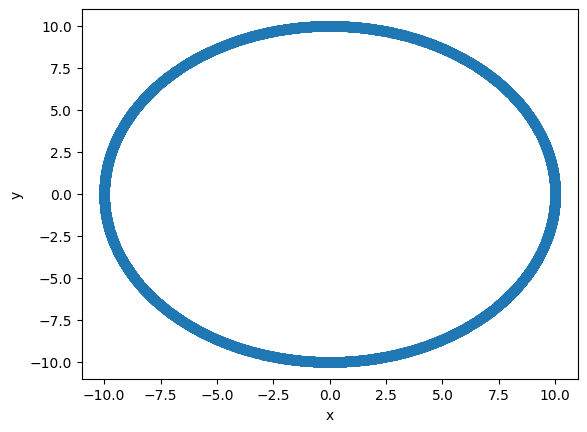
\includegraphics[width=\linewidth]{images/d-zbior-b.png}
		\verb|generate_circle_points((0, 0), 10, 10**4)|
		\caption*{Rysunek zbiór T.B}
	\end{subfigure}
\end{figure}

\begin{figure}[htp]
	\begin{subfigure}[t]{.45\textwidth}
		\centering
		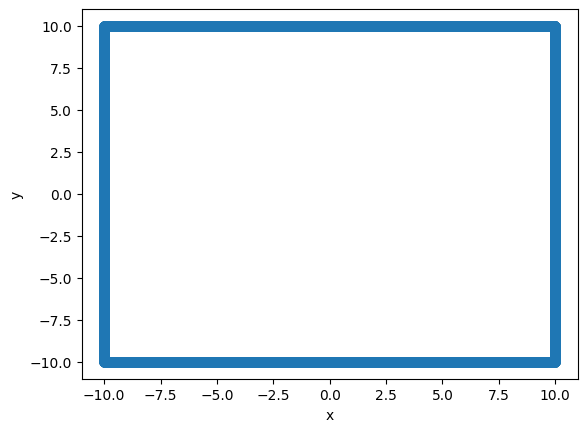
\includegraphics[width=\linewidth]{images/d-zbior-c.png}
		\verb|generate_rectangle_points(|
		\verb|(-10, -10), (10, -10), (10, 10), (-10, 10),|
		\verb|10**6)|
		\caption*{Rysunek zbiór T.C}
	\end{subfigure}
	\hfill
	\begin{subfigure}[t]{.45\textwidth}
		\centering
		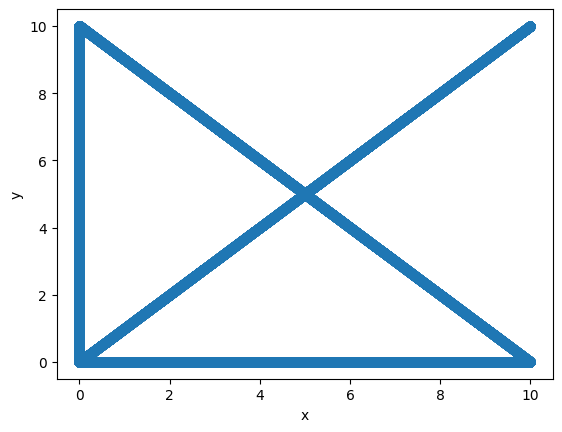
\includegraphics[width=\linewidth]{images/d-zbior-d.png}
		\verb|generate_square_points(|
		\verb|(0, 0), (10, 0), (10, 10), (0, 10),|
		\verb|10**5, 10**5)|
		\caption*{Rysunek zbiór T.D}
	\end{subfigure}
\end{figure}

\paragraph{Czas działania:}
\mbox{}
\begin{table}[H]
	\centering
	\begin{tabular}{|l|l|l|l|l|}
		\hline
		\textbf{Algorytm} & \textbf{Zbiór T.A} & \textbf{Zbiór T.B} & \textbf{Zbiór T.C} & \textbf{Zbiór T.D} \\ \hline
		Graham & 1.5 s & 3.1 s & 1.3 s & 4.9 s \\ \hline
		Jarvis & 1.4 s & 30.9 s & 0.6 s & 1.3 s \\ \hline
	\end{tabular}
	\caption*{Tabela 1 Czasy działania}
\end{table}


\newpage

\section*{Wnioski}
\subsection*{Wspólne dla obu algorytmów}
$\bullet$ Oba służą do znajdowania otoczki wypukłej

\subsection*{Algorytm grahama}
$\bullet$ Złożoność O(n log n) - (n to liczba punktów)


$\bullet$ Wyniki są wrażliwe na rozkład punktów, co spowodowane jest porównywaniem ich względem kąta który tworzą z osią OX (Widzimy to szczególnie w przypadku przekątnych kwadratu, gdzie jedna przekątna została potraktowana poprawnie jako punkty współliniowe, ale za to prawie cała druga przekątna była i tak sprawdzana).


$\bullet$ Jest zazwyczaj szybszy dla ogólnych danych, ale nie intuicyjnie na wyniki wpływa dokładność obliczeń, na co należy zwrócić uwagę.

\subsection*{Algorytm jarvisa}
$\bullet$ Jego złożoność O(n * k) - zależna od rozmiaru rozwiązania (k to ilość punktów otoczki)


$\bullet$ Idea działania algorytmu jest intuicyjna


$\bullet$ Jak pokazuje przykład przekątnych prostokąta może być szybszy od algorytmu grahama


$\bullet$ Zmiana epsilona lepiej odpowiada zmianie dokładności szukania punktów.


\section*{Bibliografia}
\par
$\bullet$ Wprowadzenie do algorytmów wydanie 3, Thomas H. Cormen, Charles E. Leiserson, Ronald L. Rivest, Stein Clifford


\end{document}
